% IT-Sicherheitsarchitekturen Ausarbeitung
% Julian Bayer, Thomas Bopst, Felix Schuckert
% HTWG-Konstanz
%
% Date: SS2014
%

\documentclass[11pt,a4paper]{report}

% Own packages
\usepackage[utf8]{inputenc}
\usepackage[german]{babel}
\usepackage{courier}
\usepackage{listings}
%\lstset{numbers=left, numberstyle=\tiny, numbersep=20pt} % Programmcode einfügen
\lstset{basicstyle=\footnotesize\ttfamily, breaklines=true}
\lstset{language=XML}
\lstset{inputencoding=utf8}
\selectlanguage{german}


%\usepackage[printonlyused]{acronym}
% PDF Eigenschaften
% -----------------
\usepackage
[
	colorlinks = false,
	bookmarks = true,
	pdftitle={IT-Sicherheitsarchitekturen (MSI SS14)},
	pdfauthor={Julian Bayer, Thomas Bopst, Felix Schuckert},
	pdfsubject={MSI IT-Sicherheitsarchitekturen},
	pdfkeywords={HTWG-Konstanz, IT-SEC, MSI},
	urlcolor=blue,
	pdfstartview=FitH
]{hyperref}

\usepackage{titlesec}
\titleformat{\chapter}[display]
{\normalfont\huge\bfseries}{\chaptertitlename\ \thechapter}{20pt}{\Huge}
\titlespacing*{\chapter}{0pt}{-40pt}{20pt}

% HTWG-Template
\usepackage{graphicx}
\usepackage{a4wide} % HTWG a4
%\usepackage[english]{babel}

% HTWG-Template
\newcommand{\thema}{Firewall und Client-to-Lan VPN}
\newcommand{\abgabedatum}{01.01.1900}
\newcommand{\autor}{Julian Bayer\\ Thomas Bopst\\ Felix Schuckert}

\begin{document}

% select language

 % set pagecount style to i,ii,...
\setcounter{page}{1}
\pagenumbering{roman}


% HTWG-Template
% -------------

\begin{titlepage}

\vspace*{-3.5cm}

\begin{center} %flushleft
\hspace*{-1cm} 
\includegraphics[width=15.7cm]{figures/htwg-logo}
\end{center} %flushleft

\vspace{2.5cm}

\begin{center}
	\huge{
		\textbf{\thema} \\[5cm]
	}
	\Large{
		\textbf{\autor}} \\[6.5cm]
	\large{
		\textbf{Konstanz, \abgabedatum} \\[2.3cm]
	}

	\Huge{
		\textbf{{\sf IT-Sicherheitsarchitekturen}}
	}
\end{center}

\end{titlepage}



% change language to english

% Abbreviations
%\include{chapters/abbreviation}
%\newpage

% Table of contents
\tableofcontents
\newpage
%\listoffigures
%\listoftables

% Content
% -------
\setcounter{page}{1} % set pagecount style to 1, 2, ...
\pagenumbering{arabic}

\chapter{Firewall} \label{fw}


\chapter{Client-to-LAN VPN}

\section{Aufgabenstellung}

Mitarbeiter von Firma A, sollen die Möglichkeit haben von überall arbeiten zu können und von dort auch Zugriff auf das interne Firmen Netzwerk zu erhalten.
Vorrausgesetzt wird hierbei selbstverständlich der Zugang zum Internet.

Realisiert werden soll dies mittels einer Client-to-LAN VPN-Verbindung die technisch mittels der freien Software \emph{OpenVPN} implementiert werden soll.

\section{Implementierung}

Um eine Verbindung zwischen einem externen Mitarbeiter bzw. dem externen Gerät und dem internen Netzwerk von Firma A herstellen zu können muss einerseits ein \textbf{Server} den VPN Dienst anbieten und andererseits muss der \textbf{Client} so konfiguriert sein, dass er sich mit diesem Dienst verbinden kann.
Als Server dient die innere Firewall \emph{fw2.firma-a.f223}, denn nur auf dieser besteht die Möglichkeit den VPN-Server so einzurichten, damit die sich verbindenden Clients zugriff auf das Intranet erhalten.
Beim Client handelt es sich um den externen Laptop \emph{lap01.internet.f223}.

Im Folgenden wird die Installation und Konfiguration der OpenVPN Software auf Client und Server erläutert.


\subsection{Server}

Auf dem der internen Firewall von Firma a müssen zunänchst die benötigten Software Packete installiert werden. Hierbei handelt es sich um das Packet \emph{openvpn}, welches die OpenVPN Software enthält. Zusätzlich wird noch das Packet \emph{bridge-utils} benötigt, welches zur Konfiguration der Bridge zwischen des von OpenVPN bereitgestellten Neztwerkinterfaces \emph{tap0} und dem normalen Netzwerkadapter \emph{eth0}, mit dem das Intranet verbunden ist, zu verbinden.

Die Installation der Packete erfolgt mittels der folgenden Befehle.

\begin{lstlisting}
apt-get install openvpn
apt-get install bridge-utils
\end{lstlisting}

% Screenshot der ifconfig wenn VPN gestartet ist und wenn nicht

\subsection{Client}

\chapter{Verifikation}
\section{Netzwerkkonfiguration}
Die korrekte Konfiguration des Netzwerks konnte mittels des ifconfig-Befehls geprüft werden. 

\lstinputlisting[
    firstline=1,
    lastline=29,
    label = ver:ifconfig1,
    caption={ifconfig-Ausgabe fw1.firma-a.f223}
]{code/fw1_ifconfig.txt}

Listing \ref{ver:ifconfig1} zeigt die Ausgabe des ifconfig Befehls auf der äußeren Firewall. Wie unschwer zu erkennen ist, sind die in Abb. \ref{fig:netzplan} vorgegebenen IP-Adressen (192.168.40.250 / 10.1.0.131), sowie die entsprechenden Netzwerke korrekt gesetzt (z. 2 und z. 12). Die ifconfig-Ausgabe der inneren Firewall wurde bereits in Listing \ref{vpn:ifconfig} angegeben. Auch hier kann man die korrekt gesetzten IP-Adressen erkennen, allerdings ist die ursprünglich für eth0 gesetzte IP-Adresse durch das bilden der Netzwerkbridge auf br0 übergegangen. IP-Adresse (192.168.30.240 / 192.168.40.240) und Netzwerk finden sich in z. 2 und z.20.


\section{Network-Address-Translation}
Zur Verifikation der NAT-Funktionalität war es zunächst nötig zu prüfen, ob das Forwarding zwischen den Netzwerkinterfaces funktionierte. Dazu wurde von einem Client aus dem Firmen-LAN zunächst die IP-Adresse 10.1.0.131 (Äußere Schnittstelle von fw1) gepingt, siehe Abb. \ref{fig:pc01_ping_fw1}. Anschließend wurde ein Traceroute zum Server net1.internet.f223 vorgenommen, der auch beweist, dass beide Firewalls passiert werden. Das Ergebnis ist in Abb. \ref{fig:pc01_traceroute_net1} zu sehen.

\begin{figure}[h!]
	\centering
		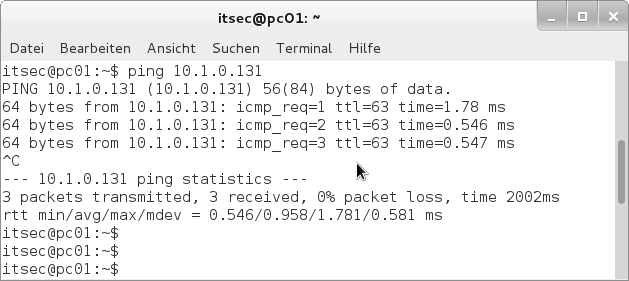
\includegraphics[width=0.7\textwidth]{figures/pc01_ping_fw1.png}
	\caption{Ping auf die äußere Schnittstelle von fw1 aus dem LAN heraus}
	\label{fig:pc01_ping_fw1}
\end{figure}


\begin{figure}[h!]
	\centering
		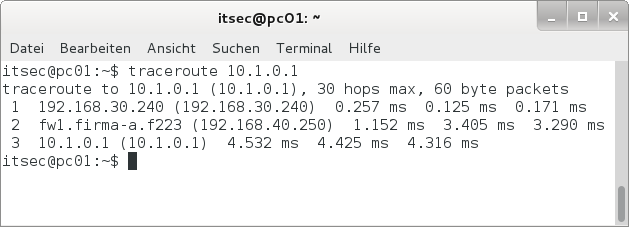
\includegraphics[width=0.7\textwidth]{figures/pc01_traceroute_net1.png}
	\caption{Traceroute aus dem LAN zu net1.internet.f223}
	\label{fig:pc01_traceroute_net1}
\end{figure}

Zum Nachweis, dass das IP-Masquerading funtioniert, wurde von pc01.firma-a.f223 ein Ping-Befehl auf 10.1.0.1 (net1.internet.f223) ausgeführt. Der Netzwerkverkehr dieses Ping-Befehls wurde jeweils in der DMZ (Abb. \ref{fig:ws_dmz}) und im Internet (Abb. \ref{fig:ws_internet}) mit Wireshark mitgeschnitten. Dabei ist sichtbar, dass die Quell-IP-Adresse beim Ping-Request jeweils mit der IP der zuletzt passierten Firewall (fw2 in der DMZ, fw1 im Internet) maskiert wurde.

\begin{figure}[h!]
	\centering
		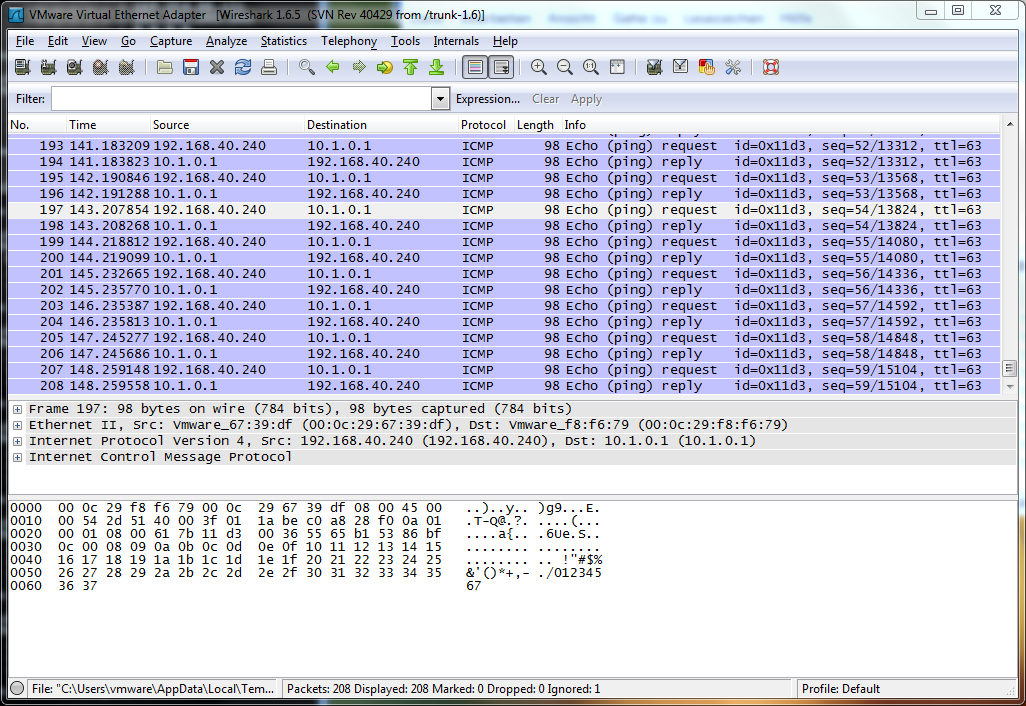
\includegraphics[width=0.7\textwidth]{figures/ws_dmz.png}
	\caption{Wireshark-Mittschnitt des Ping in der DMZ}
	\label{fig:ws_dmz}
\end{figure}

\begin{figure}[h!]
	\centering
		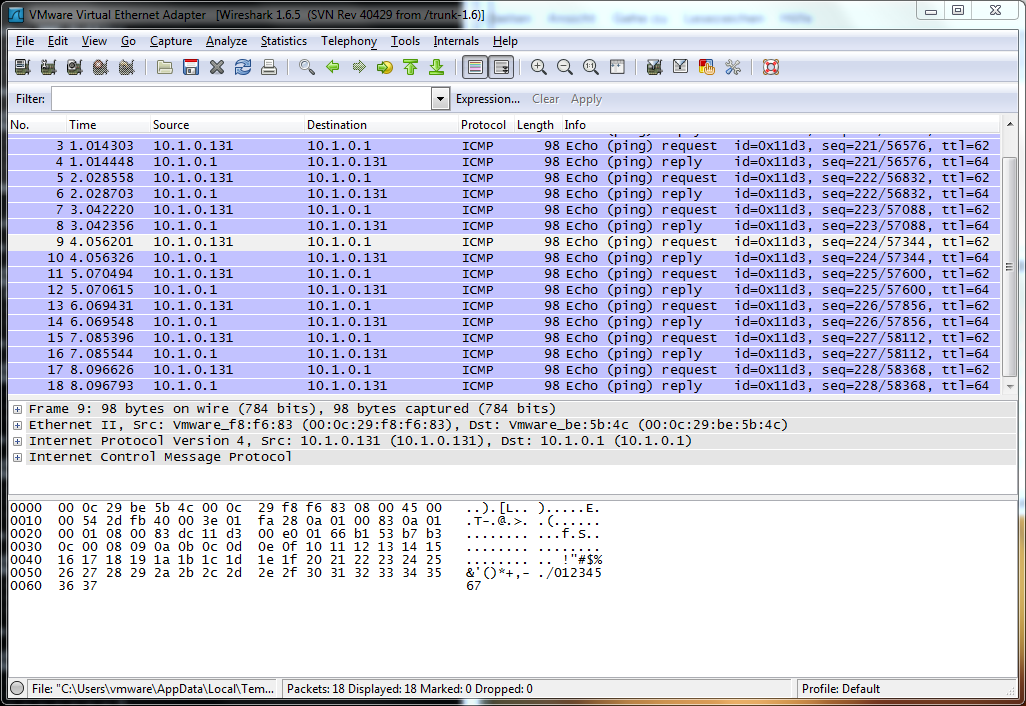
\includegraphics[width=0.7\textwidth]{figures/ws_internet.png}
	\caption{Wireshark-Mittschnitt des Ping im Internet}
	\label{fig:ws_internet}
\end{figure}

Das korrekte Port-Forwarding der Dienste Webserver, Mailserver und VPN-Server, das am äußeren Server eingerichtet werden musste, konnte durch Nutzung der entsprechenden Dienste auf lap01.internet.f223 verifiziert werden.

\section{VPN}
Die Korrektheit der VPN-Konfiguration wurde folgendermaßen getestet:

\paragraph{Konnektivität zum Mailserver}
Mit Hilfe des installierten Mail-Clients wurde überprüft, dass E-Mails empfangen und gesendet werden können, einerseits mit aktiver VPN-Verbindung, sowie ohne VPN-Verbindung.

\paragraph{Erreichbarkeit der Webserver}
Die Erreichbarkeit der Webserver wurde durch aufrufen der URL des net1.internet.f223, im installierten Webbrowser, verifiziert. Hierbei wurde geprüft, ob die Webseite, einerseits mit aktiver und mit nicht aktiver VPN-Verbindung, aufgerufen werden kann.

Des Weiteren wurde geprüft, ob die Website auf dem internen Webserver srv01.firma-a.f223 aufgerufen werden kann. Dies ist korrekterweise mit der URL srv01.firma-a.f223 nur mit aktiver VPN-Verbindung möglich, da der DNS-Eintrag nur im DNS-Server von Firma a bekannt ist, jedoch nicht im Internet.

\paragraph{Erreichbarkeit der Rechner im Intranet}
Zudem wurde geprüft, ob bei bestehender VPN-Verbindung der Computer pc01.firma-a.f223 im Firmen-Intranet erreichbar ist. Dies wurde mit Hilfe des Programms \texttt{ping} verifiziert. Abbildung \ref{vpn:lap01-ping-pc01} zeigt die Erreicharkeit von pc01 von lap01 und Abbildung \ref{vpn:pc01-ping-lap01} zeigt die umgekehrte Erreichbarkeit.

\begin{figure}[h!]
  \centering
    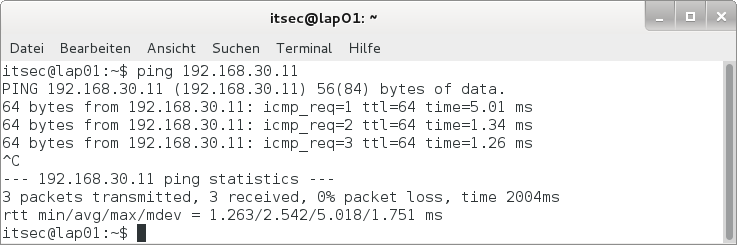
\includegraphics[width=0.7\textwidth]{figures/vpn_lap01_ping_pc01.png}
  \caption{Ping von lap01.internet.f223 mit aktiver VPN zu pc01.firma-a.f223}
  \label{vpn:lap01-ping-pc01}
\end{figure}

\begin{figure}[h!]
  \centering
    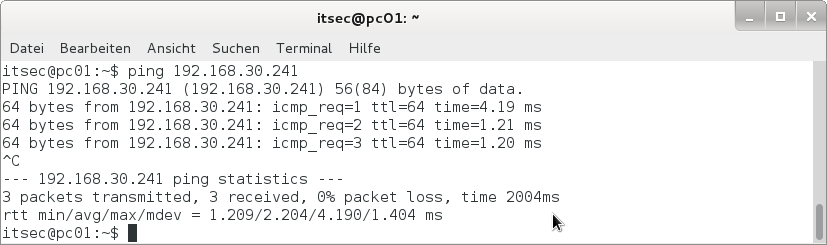
\includegraphics[width=0.7\textwidth]{figures/vpn_pc01_ping_lap01.png}
  \caption{Ping von pc01.firma-a.f223 zu lap01.internet.f223 mit aktiver VPN}
  \label{vpn:pc01-ping-lap01}
\end{figure}

\paragraph{Verschlüsselung der VPN-Verbindung}

\begin{figure}[h!]
  \centering
    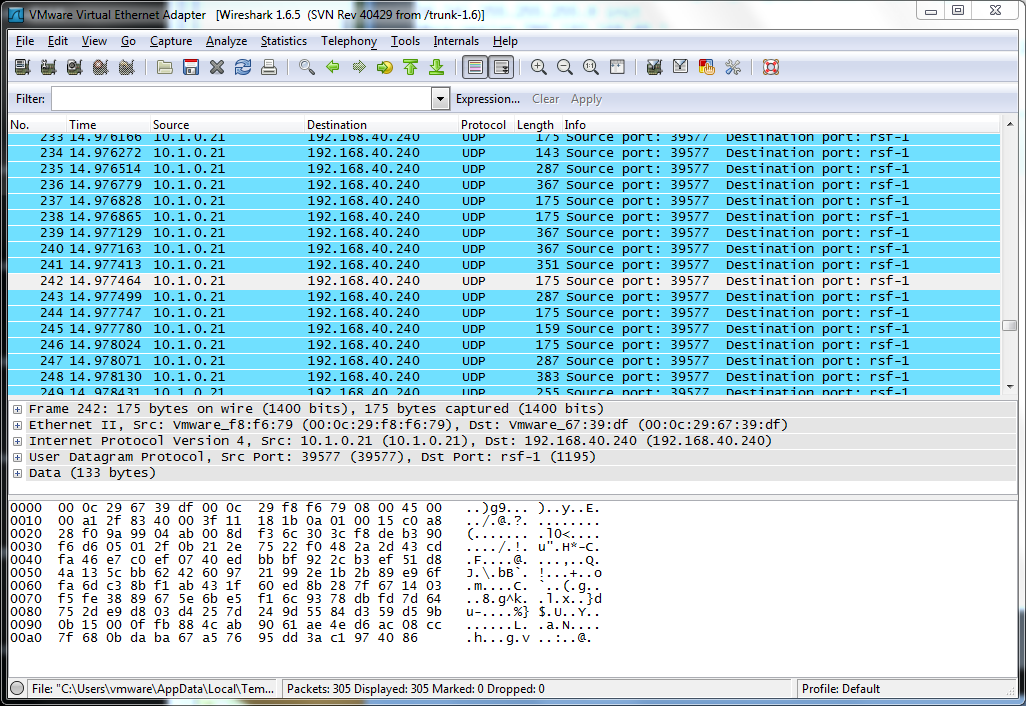
\includegraphics[width=0.7\textwidth]{figures/vpn_ws_lap01_ping_pc01.png}
  \caption{Mitschnitt des Pings von lap01.internet.f223 mit aktiver VPN zu pc01.firma-a.f223}
  \label{vpn:ws_lap01-ping-pc01}
\end{figure}


Um zeigen zu können, dass die Verschlüsselung der VPN-Verbindung funktioniert, wurde ein Mitschnitt der Ping-Nachricht, von lap01 mit aktiver VPN-Verbindung zu pc01, mit Hilfe des Programms Wireshark aufgezeichnet.
Abbildung \ref{vpn:ws_lap01-ping-pc01} zeigt dabei ein Paket des Pings. Hierbei lässt sich gut die Konfiguration erkennen. Als Übertragungsprotokoll wurde UDP verwendet, was die Abbildung bestätigt. Des Weiteren lässt sich zeigen, dass die Pakete von lap01 mit dessen öffentlicher IP-Adresse \texttt{10.1.0.21} von einem beliebigen Port \texttt{39577} an den VPN-Server mit der Adresse (DMZ) \texttt{192.168.40.240} an Port \texttt{1195}, welches der konfigurierte Port ist, gesendet werden. Das eigentliche ICMP-Paket an pc01, kann hierbei nicht erkannt werden, da es sich verschlüsselt in diesem Paket befindet.

\paragraph{DNS-Server-Konfiguration}

\begin{figure}[h!]
  \centering
    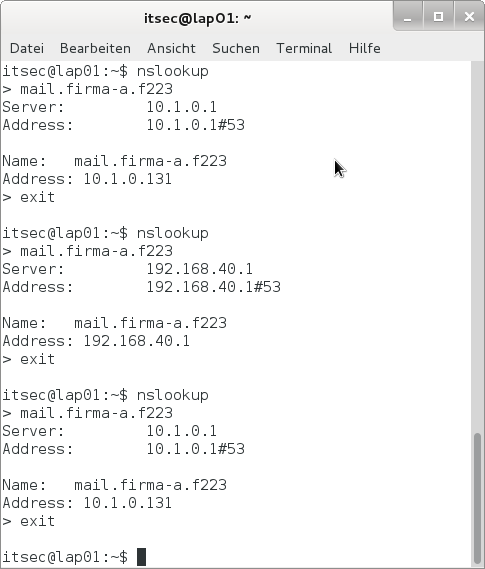
\includegraphics[width=0.5\textwidth]{figures/vpn_nslookup.png}
  \caption{Verifikation der DNS-Server-Konfiguration beim aktivieren der VPN-Verbindung.}
  \label{vpn:lap01_nslookup}
\end{figure}

Abschließend wurde noch die DNS-Server-Konfiguration geprüft, denn wie bereits in Kapitel \ref{vpn:client} erwähnt, soll bei aktiver VPN-Verbindung der Firmeneigene DNS-Server, der sich auf srv01.firma-a.f223 in der DMZ befindet, verwendet werden. Bei nicht aktiver VPN-Verbindung soll der im System konfigurierte DNS-Server auf net1.internet.f223 genutzt werden.

Dies kann mit Hilfe des Programms \texttt{nslookup} verifiziert werden. Der erste, sowie der letzte Aufruf in Abbildung \ref{vpn:lap01_nslookup} erfolgte jeweils mit nicht aktiver VPN-Verbindung. Zum Test wurde die Domain \texttt{mail.firma-a.f223} verwendet, welche in beiden genannten DNS-Servern eingetragen ist.

Hierbei lässt sich erkennen, dass bei nicht aktiver VPN jeweils der DNS-Server mit der IP-Adresse 10.1.0.1 verwendet wurde, also der net1 Server. Des Weiteren lässt sich erkennen, dass dieser die Domain auf die äußere IP-Adresse von fw1 auflöst, was korrekt ist.

Der mittlere Eintrag wurde mit aktiver VPN-Verbindung durchgeführt. Hierbei lässt sich erkennen, dass diesmal der Firmeneigenen DNS-Server mit der IP-Adresse \texttt{192.168.40.1} verwendet wird. Zudem löst der DNS-Server die Domain ebenfalls auf diese IP-Adresse auf, da sich der Webserver auf dem gleichen Server befindet.

Durch diese drei Aufrufe wird bestätigt, dass das Ändern und wieder Rückgängig machen, der Änderung des DNS-Servers, beim Aktivieren und Deaktivieren der VPN-Verbindung, funktioniert.



%\appendix
%\include{chapters/appendix}

\addcontentsline{toc}{chapter}{Literaturverzeichnis} %References
\bibliographystyle{IEEEtranS}
\bibliography{bib/references}

\end{document}
